\section{\emph{Retriever}}
\label{sec:retriever_exp}
Μελετήθηκαν δύο μοντέλα \emph{Retriever}, το \emph{TF-IDF} και το \emph{BM25}. Τα μοντέλα παίρνουν ως είσοδο τις ερωτήσεις του συνόλου δεδομένων και αξιολογούνται στο αν σε κάποιο από έγγραφα επιστροφής περιέχεται η σωστή απάντηση, δηλαδή αν η απάντηση βρίσκεται στο πρώτο, στο πρώτο ή στο δεύτερο, στο πρώτο ή στο δεύτερο ή στο τρίτο και ούτω καθεξής μέχρι και τα δέκα έγγραφα. Με τον τρόπο αυτό βελτιστοποιείται ο αριθμός εγγράφων που επιστρέφονται στον \emph{Reader}. Επιπλέον, σε αυτό το σημείο αξίζει να σημειωθεί ότι ο αριθμός των εγγράφων που επιστρέφονται δεν πρέπει να είναι πολύ μεγάλος διότι τότε η διαδικασία εύρεσης της απάντησης από τον \emph{Reader} θα χρειάζεται απελπιστικά μεγάλο χρόνο.
% , \ref{tfidf-acc}
Στα σχήμα \ref{bm25-acc} παρουσιάζονται τα αποτελέσματα για τα δύο μοντέλα. Είναι φανερό ότι το \emph{BM25} υπερτερεί του \emph{TF-IDF}, οπότε είναι και αυτό που επιλέχθηκε για το τελικό σύστημα. Ο αριθμός των εγγράφων που θα επιστρέφονται είναι $3$, τόσο γιατί η ακρίβεια στην επιστροφή ενός ή δύο εγγράφων ήταν συγκριτικά χαμηλότερη όσο και γιατί η επιστροφή τεσσάρων και πάνω δεν αποδίδει σημαντικά καλύτερα και θα καθυστερούσε τη διαδικασία "ανάγνωσης" από τον \emph{Reader}.


\begin{figure}[htb]
  \centering
  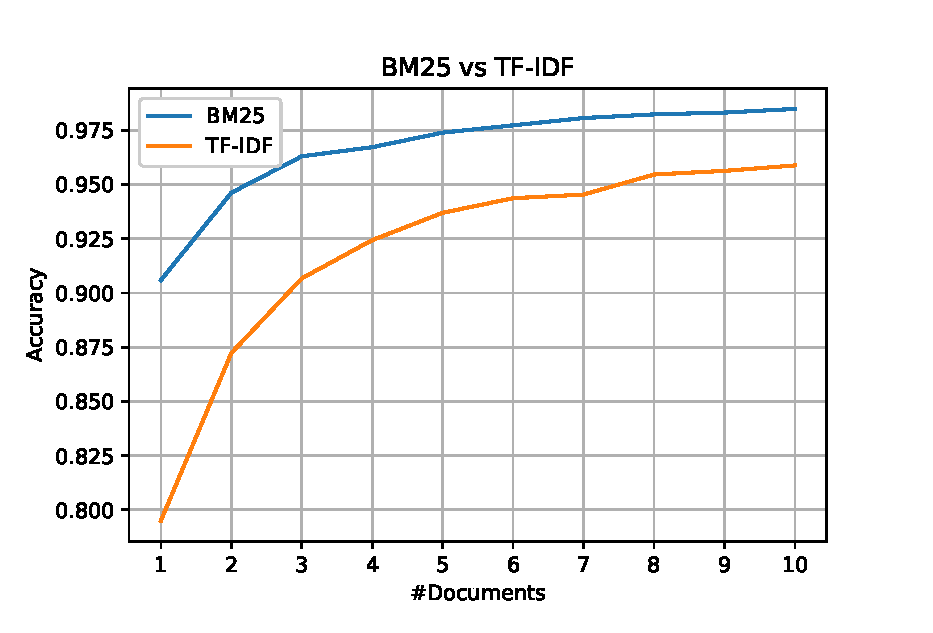
\includegraphics[width=\linewidth]{figures/chapter6/test.eps}
  \caption{Ακρίβεια \emph{BM25 Retriever} και \emph{TF-IDF Retriever} στο \emph{SQuAD} σύνολο δεδομένων}
  \label{bm25-acc}
\end{figure}

% \begin{figure}[htb]
%   \centering
%   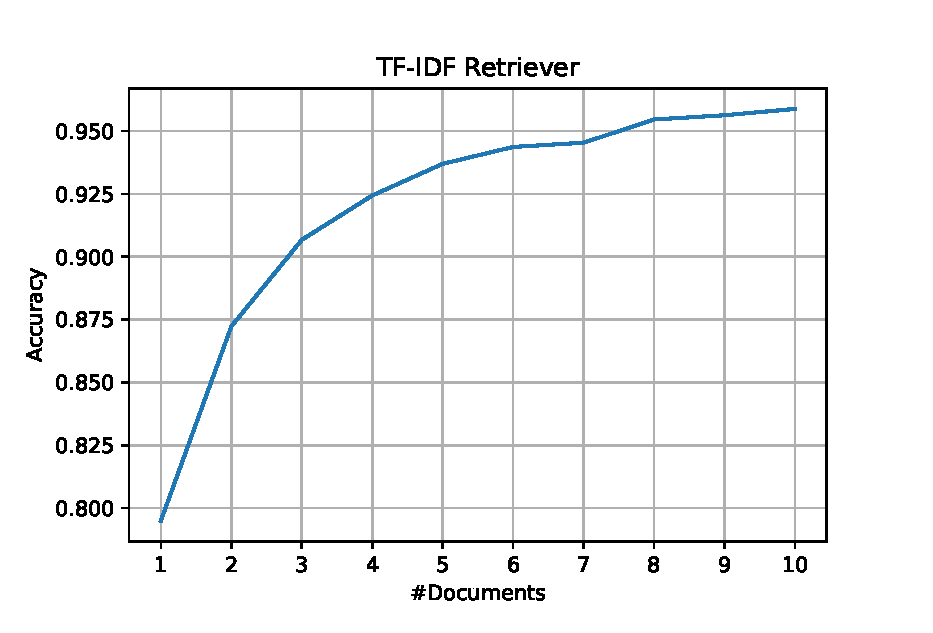
\includegraphics[width=\linewidth]{figures/chapter6/tf-idf-acc.eps}
%   \caption{Ακρίβεια \emph{TF-IDF Retriever} στο \emph{SQuAD} σύνολο δεδομένων}
%   \label{tfidf-acc}
% \end{figure}